\documentclass[12pt,a4paper]{scrartcl}
\usepackage[utf8]{inputenc}
\usepackage[english,russian]{babel}
\usepackage{misccorr}
\usepackage{graphicx}
\usepackage{amsmath}
\usepackage{amsfonts}
\usepackage{verbatim}
\usepackage{listings}
\usepackage{pgfplots}
\usepackage{graphicx}
\usepackage{pdfpages}
\usepackage{multirow}
\usepackage{booktabs}

\DeclareUnicodeCharacter{03BC}{\ensuremath{\mu}}
\DeclareUnicodeCharacter{03B3}{\ensuremath{\gamma}}
\DeclareUnicodeCharacter{03C3}{\ensuremath{\sigma}}
\DeclareUnicodeCharacter{03B8}{\ensuremath{\theta}}
\DeclareUnicodeCharacter{03C7}{\ensuremath{\chi}}
\DeclareUnicodeCharacter{03B1}{\ensuremath{\alpha}}


\usepackage{algorithm}
\usepackage{algpseudocode}

% Настройки листингов.
% 8 Листинги

\usepackage{listings}

% Значения по умолчанию
\lstset{
  language=[Sharp]C,
  basicstyle= \footnotesize,
  breakatwhitespace=true,% разрыв строк только на whitespacce
  breaklines=true,       % переносить длинные строки
%   captionpos=b,          % подписи снизу -- вроде не надо
  inputencoding=koi8-r,
  numbers=left,          % нумерация слева
  numberstyle=\footnotesize,
  showspaces=false,      % показывать пробелы подчеркиваниями -- идиотизм 70-х годов
  showstringspaces=false,
  showtabs=false,        % и табы тоже
  stepnumber=1,
  tabsize=4,              % кому нужны табы по 8 символов?
  frame=single,
  commentstyle=\color{green},
  morekeywords={partial, var, value, get, set},
  keywordstyle=\color{blue},
  stringstyle=\color{red}
}

% Стиль для псевдокода: строчки обычно короткие, поэтому размер шрифта побольше
\lstdefinestyle{pseudocode}{
  basicstyle=\small,
  keywordstyle=\color{black}\bfseries\underbar,
  language=Pseudocode,
  numberstyle=\footnotesize,
  commentstyle=\footnotesize\it
}

% Стиль для обычного кода: маленький шрифт
\lstdefinestyle{realcode}{
  basicstyle=\scriptsize,
  numberstyle=\footnotesize
}

% Стиль для коротких кусков обычного кода: средний шрифт
\lstdefinestyle{simplecode}{
  basicstyle=\footnotesize,
  numberstyle=\footnotesize
}

% Стиль для BNF
\lstdefinestyle{grammar}{
  basicstyle=\footnotesize,
  numberstyle=\footnotesize,
  stringstyle=\bfseries\ttfamily,
  language=BNF
}

% Определим свой язык для написания псевдокодов на основе Python
\lstdefinelanguage[]{Pseudocode}[]{Python}{
  morekeywords={each,empty,wait,do},% ключевые слова добавлять сюда
  morecomment=[s]{\{}{\}},% комменты {а-ля Pascal} смотрятся нагляднее
  literate=% а сюда добавлять операторы, которые хотите отображать как мат. символы
    {->}{\ensuremath{$\rightarrow$}~}2%
    {<-}{\ensuremath{$\leftarrow$}~}2%
    {:=}{\ensuremath{$\leftarrow$}~}2%
    {<--}{\ensuremath{$\Longleftarrow$}~}2%
}[keywords,comments]

% Свой язык для задания грамматик в BNF
\lstdefinelanguage[]{BNF}[]{}{
  morekeywords={},
  morecomment=[s]{@}{@},
  morestring=[b]",%
  literate=%
    {->}{\ensuremath{$\rightarrow$}~}2%
    {*}{\ensuremath{$^*$}~}2%
    {+}{\ensuremath{$^+$}~}2%
    {|}{\ensuremath{$|$}~}2%
}[keywords,comments,strings]

% Подписи к листингам на русском языке.
\renewcommand\lstlistingname{Листинг}
\renewcommand\lstlistlistingname{Листинги}


\begin{document}
\begin{titlepage}
\newpage
\begin{figure}[H]
	\centering
	\includegraphics[width=\linewidth]{"C:/Users/Barsi/Desktop/University/3 course/6sem/MathModeling/2 - Runge Kutta/Отчет/head"}
\end{figure}

\vspace{5cm}
\begin{center}
\Large Отчёт по лабораторной работе №2 \\ По дисциплине «Математическое моделирование» \\ Тема: «Программно - алгоритмические реализации методов Рунге-Кутта 2-го и 4-го порядков точности при решении системы ОДУ в задаче Коши» 
\end{center}
%\vspace{2.5em}
\vspace{6em}
\begin{flushright}
Студент: \hrulefill Барсуков Н.М. \\
\vspace{1.5em}
Группа: \hrulefill ИУ7-66\\
\vspace{1.5em}
Преподаватель: \hrulefill Градов В.М\\
\vspace{1.5em}
\end{flushright}
\vspace{\fill}
\begin{center}
Москва, 2020
\end{center}
\end{titlepage}
\newpage
\tableofcontents
\addcontentsline{toc}{section}{Введение}

\newpage
\section{Аналитический раздел}
	В данном разделе находится цель работы, описаны исходные данные, приведены методы Рунге-Кутта 1 и 2 порядка
\textbf{Цель работы:} Получение навыков разработки алгоритмов решения задачи Коши при реализации моделей, построенных на системе ОДУ, с использование методов Рунге-Кутта 2-го и 4-го порядков точности

\subsection{Исходные данные}
\begin{enumerate}
	\item Задана система электротехнических уравнений, описывающих разрядный контур, включающий постоянное активное сопротивление $R_k$ нелинейное сопротивление $R_p(I)$, завичящее от тока $I$, индуктивность $L_k$ и емкость $C_k$
	
	\begin{math}
		\left\{
			\frac{dI}{dT} = \frac{U - (R_k + R_p(I))I}{L_k} \
			\frac{dU}{dt} = - \frac{I}{C_k}
		\right\}
	\end{math}
	
	\item Начальные условия: t = 0, I = $I_0$, U = $U_0$ где I $U0$ - ток и напряжение в конденсаторе
	\item Сопротивление $R_p$ рассчитать по формуле: $R_p = \frac{I_p}{2 \pi R^2 \int_{0}^{1}\sigma(T(z))zdz}$
	\item Для функции $T(z)$ применить выражение $T(z) = T_0 + (T_w - T_0)z^m$ параметры $T_0, m$ находятся интерполяцией из табл \ref{tab:l} при известном токе I.
	Коэффиицент электропроводности $\sigma(T)$ зависит от T и рассчитывается интерполяцией из \ref{tab:2}.
	\item \begin{enumerate}
		\item R = 0.35m
		\item $l_e$ = 12cm
		\item $L_k$ = $187 * 10^{-6}$Гн
		\item $C_k$ = $268 * 10^{-6}$Ф
		\item $Rk$ = 0.25Om
		\item $U_co$ = 1400В
		\item $I_0$ = 0.3A
		\item $Tw$ = 2000k
	\end{enumerate}
\end{enumerate}
	
	% Table generated by Excel2LaTeX from sheet 'Лист1'
	\begin{table}[H]
		\centering
		\caption{Таблица 1}
		\begin{tabular}{|c|p{4.215em}|}
			\toprule
			\multicolumn{1}{|p{4.215em}|}{T, K} & , 1/Ом см \\
			\midrule
			4000,00 & 0.031 \\
			\midrule
			5000,00 & 0.27 \\
			\midrule
			6000,00 & \multicolumn{1}{c|}{43953,00} \\
			\midrule
			7000,00 & \multicolumn{1}{c|}{43988,00} \\
			\midrule
			8000,00 & 12.0 \\
			\midrule
			9000,00 & \multicolumn{1}{c|}{44093,00} \\
			\midrule
			10000,00 & \multicolumn{1}{c|}{44011,00} \\
			\midrule
			11000,00 & 41.1 \\
			\midrule
			12000,00 & 54.1 \\
			\midrule
			13000,00 & 67.7 \\
			\midrule
			14000,00 & 81.5 \\
			\bottomrule
		\end{tabular}%
		\label{tab:l}%
	\end{table}%

	% Table generated by Excel2LaTeX from sheet 'Лист1'
	\begin{table}[H]
		\centering
		\caption{Таблица 2}
		\begin{tabular}{|c|c|c|}
			\toprule
			\multicolumn{1}{|p{4.215em}|}{I, A} & \multicolumn{1}{p{4.215em}|}{To, K} & \multicolumn{1}{p{4.215em}|}{m} \\
			\midrule
			\multicolumn{1}{|p{4.215em}|}{0.5} & 6730,00 & \multicolumn{1}{p{4.215em}|}{0.50} \\
			\midrule
			1,00  & 6790,00 & \multicolumn{1}{p{4.215em}|}{0.55} \\
			\midrule
			5,00  & 7150,00 & 1,70 \\
			\midrule
			10,00 & 7270,00 & 3,00 \\
			\midrule
			50,00 & 8010,00 & 11,00 \\
			\midrule
			200,00 & 9185,00 & 32,00 \\
			\midrule
			400,00 & 10010,00 & 40,00 \\
			\midrule
			800,00 & 11140,00 & 41,00 \\
			\midrule
			1200,00 & 12010,00 & 39,00 \\
			\bottomrule
		\end{tabular}%
		\label{tab:2}%
	\end{table}%

\subsection {Рунге-Кутта 2ого порядка}
	\begin{equation*}
		\begin{cases}
			I_{n + 1} = & I_n + h_n[(1 - \alpha)f(\Delta t, I_n, U_n) + \alpha f(x_n + \frac{h_n}{2\alpha}, I_n + \frac{h_n}{2\alpha}f(\Delta t, I_n, U_n), U_n + \frac{h-n}{2\alpha}\phi(\Delta t, I_n, U_n))] \\
			U_{n + 1} = &  Un + h_n[(1 - \alpha)\phi(\Delta t, I_n, U_n) + \alpha\phi(x_n + \frac{h_n}{2\alpha}, I_n + \frac{h_n}{2\alpha}f(\Delta t, I_n, U_n), U_n + \frac{h_n}{2\alpha}\phi(x_n + \frac{h_n}{2\alpha}))] \\
		\end{cases}
	\end{equation*}, где $\alpha$ = (0.5, 1)
	
\subsection{Рунге-Кутта 4ого порядка}
	\begin{equation*}
		I_{n + 1} = I_n + \Delta t\frac{k_1+2k_2+2k_3+k_4}{6}
	\end{equation*}
	\begin{equation*}
		U_{n_1} = U_n + \Delta t \frac{q_1 + 2q_2 + 2q_3 + q_4}{6}
	\end{equation*}
	
	\begin{equation*}
		\begin{cases}
			k_1= & h_nf(\delta t, I_n, U_n) \\
			q_1= & h_n\phi(\delta t, I_n, U_n) \\
			k_2= & h_nf(\delta t + \frac{h_n}{2}, I_n + \frac{k_1}{2}, U_n + \frac{q_1}{2}) \\
			q_2= & h_n\phi(\delta t + \frac{h_n}{2}, I_n + \frac{k_1}{2}, U_n + \frac{q_1}{2}) \\
			k_3= & h_nf(\delta t + \frac{h_n}{2}, I_n + \frac{k_2}{2}, U_n + \frac{q_2}{2}) \\
			q_3= & h_n\phi(\delta t + \frac{h_n}{2}, I_n + \frac{k_2}{2}, U_n + \frac{q_1}{2}) \\
			k_4= & h_nf(\Delta t + h_n, I_n = k_3, U_n + q_3) \\ 
			q_4= & h_n\phi(\Delta t + h_n, I_n + k_3, U_n + q_3 ) \\
		\end{cases}
	\end{equation*}
	
\section{Технологический раздел}
	В данном разделе указаны минимальные системные требования. Описан используемый язык и среда разработки. 
	Приведен листинг программы.
	
	\subsection{Минимальные требования}
	 	Минимальные системные требования: PC с операционной системой Windows 7/8/10. 
	 	Требуется устройство ввода: клавиатура, мышь.
	 	Устройства вывода: монитор
	 	
	\subsection{Выбор языка и среды разработки}
		Для достижения поставленной цели, мной был выбран язык Python версии 3.6 по причине удобства для математических вычислений, так же из за болеее лучшего уровня знания данного языка.
		Использовался sublime и интерпретатор для python.
		
	\subsection{Листинг}
	\begin{lstlisting}[]
import math
import numpy
import matplotlib.pyplot as plt
from decimal import Decimal

R = 0.35
Tw = 2000.0
Ck = 268e-6
Lk = 187e-6
Rk = 0.25  #0.5 to= 200
Uc0 = 1400.0
I0 = 0.5  #0.5 to 3
le = 12.0
I4 = I0
Uc4 = Uc0
I2 = I0
Uc2 = Uc0
T0 = 0.0
m = 0.0

masI = [0.5, 1, 5, 10, 50, 200, 400, 800, 1200]
masT0 = [6730, 6790, 7150, 7270, 8010, 9185, 
		10010, 11140, 12010]
masm = [0.5, 0.55, 1.7, 3, 11, 32, 40, 41, 39]
masT = [4000, 5000, 6000, 7000, 8000, 9000, 
		10000, 11000, 12000, 13000, 14000]
masSigm = [0.031, 0.27, 2.05, 6.06, 12.0, 19.9, 
			29.6, 41.1, 54.1, 67.7, 81.5]


def f(xn, yn, zn, m_Rp):
	return -((Rk + m_Rp) * yn - zn)/Lk


	def phi(xn, yn, zn):
	return -yn/Ck


def trapez(start, end, function):
	step = 0.05#(end - start)/20
	result = 0
	while start <= end:
	left = function(start)
	start += step
	right = function(start)
	result += step*(left + right)/2
	return round(result, 4)


def integrate_polynom(coefs):
	result = [0]
	for i in range (len(coefs)):
	result.append(coefs[i - 1]/i)
	return result


def polynom_value(coefs, x):
	result = 0
	degree = 1
	for i in range(len(coefs)):
	if(coefs[i] != 0):
	result += coefs[i] * degree
	degree *= x
	return result

def interpolate(x, x_arr, y_arr):
	i = 0
	if (x <= x_arr[0]):
		x0 = x_arr[0]
		x1 = x_arr[1]
		y0 = y_arr[0]
		y1 = y_arr[1]
	elif (x > x_arr[-1]):
		x0 = x_arr[-2]
		x1 = x_arr[-1]
		y0 = y_arr[-2]
		y1 = y_arr[-1]
	else:
		while(x >= x_arr[i]):
			x0 = x_arr[i - 1]
			x1 = x_arr[i]
			y0 = y_arr[i - 1]
			y1 = y_arr[i]
			i += 1
	return y0 + (y1 - y0) * x / (x1 - x0)


def T(z, m, T0):
	return T0 + (Tw -T0) * z**m


def sigma(T):
	return interpolate(T, masT, masSigm)


def rp(I):
	m = interpolate(I, masI, masm)
	T0 = interpolate(I, masI, masT0)
	integ = trapez(0, 1, lambda z: sigma(T(z, m, T0)) * z)
	return le / (2 * math.pi * R*R * integ), T0


def second_order(xn, yn, zn, hn, m_Rp):
	alpha = 1
	yn_1 = yn + hn * ((1 - alpha) * f(xn, yn, zn, m_Rp) + alpha \
	* f(xn + hn/(2*alpha),
	yn + hn/(2*alpha) * f(xn, yn, zn, m_Rp),
	zn + hn/(2*alpha) * phi(xn, yn, zn), m_Rp))
	zn_1 = zn + hn * ((1 - alpha) * phi(xn, yn, zn) + alpha \
	* phi(xn + hn/(2*alpha),
	yn + hn/(2*alpha) * f(xn, yn, zn, m_Rp),
	zn + hn/(2*alpha) * phi(xn, yn, zn)))
	return yn_1, zn_1


def fourth_order(xn, yn, zn, hn, m_Rp):
	k1 = hn * f(xn, yn, zn, m_Rp)
	q1 = hn * phi(xn, yn, zn)
	k2 = hn * f(xn + hn/2, yn + k1/2, zn + q1/2, m_Rp)
	q2 = hn * phi(xn + hn/2, yn + k1/2, zn + q1/2)
	
	k3 = hn * f(xn + hn/2, yn + k2/2, zn + q2/2, m_Rp)
	q3 = hn * phi(xn + hn/2, yn + k2/2, zn + q2/2)
	
	k4 = hn * f(xn + hn, yn + k3, zn + q3, m_Rp)
	q4 = hn * phi(xn + hn, yn + k3, zn + q3)
	
	yn_1 = yn + (k1 + 2*k2 + 2*k3 + k4)/6
	zn_1 = zn + (q1 + 2*q2 + 2*q3 + q4)/6
	return yn_1, zn_1


def do_plot(pltMasT, mas1, mas2, xlabel, 
			ylabel, name1, name2):
	plt.plot(pltMasT, mas1)
	plt.plot(pltMasT, mas2)
	plt.xlabel(xlabel)
	plt.ylabel(ylabel)
	plt.legend((name1, name2))
	plt.grid(True)
	plt.show()


if __name__ == "__main__":
	pltMasT = []
	pltMasI4 = []
	pltMasU4 = []
	pltMasRp4 = []
	pltMasI2 = []
	pltMasU2 = []
	pltMasRp2 = []
	pltMasT0 = []
	pltMasT1 = []
	h = 1e-6
for t in numpy.arange(0, 20e-6, h):
	try:
	m_Rp4, T0 = rp(I4)
	m_Rp2, T1 = rp(I2)
	
	#if t > h:
	pltMasT0.append(T0)
	pltMasT1.append(T1)
	
	pltMasT.append(t)
	pltMasI4.append(I4)
	pltMasU4.append(Uc4)
	pltMasRp4.append(m_Rp4)
	pltMasI2.append(I2)
	pltMasU2.append(Uc2)
	pltMasRp2.append(m_Rp2)

	I4, Uc4 = fourth_order(t, I4, Uc4, h, m_Rp4)
	I2, Uc2 = second_order(t, I2, Uc2, h, m_Rp2)
	except Exception as e:
	print(e)
	except:
		break


do_plot(pltMasT, pltMasI4, pltMasI2, 't', 
		'I', '4th order', '2nd order')
do_plot(pltMasT, pltMasU4, pltMasU2, 't', 
		'Uc', '4th order','2nd order')
do_plot(pltMasT, pltMasRp4, pltMasRp2,'t', 
		'Rp', '4th order', '2nd order')

for i in range(len(pltMasI4)):
	pltMasI4[i] *= pltMasRp4[i]
	pltMasI2[i] *= pltMasRp2[i]

do_plot(pltMasT, pltMasI4, pltMasI2, 't', 
		'I * Rp', '4th order', '2nd order')
do_plot(pltMasT, pltMasT0, pltMasT1, 't', 
		'T0', '4th order', '2nd order')
	\end{lstlisting}
	
	\subsection{Результаты работы программы}
	В данном подразделе приводятся результаты работы программы
	
	\begin{figure}[H]
		\centering
		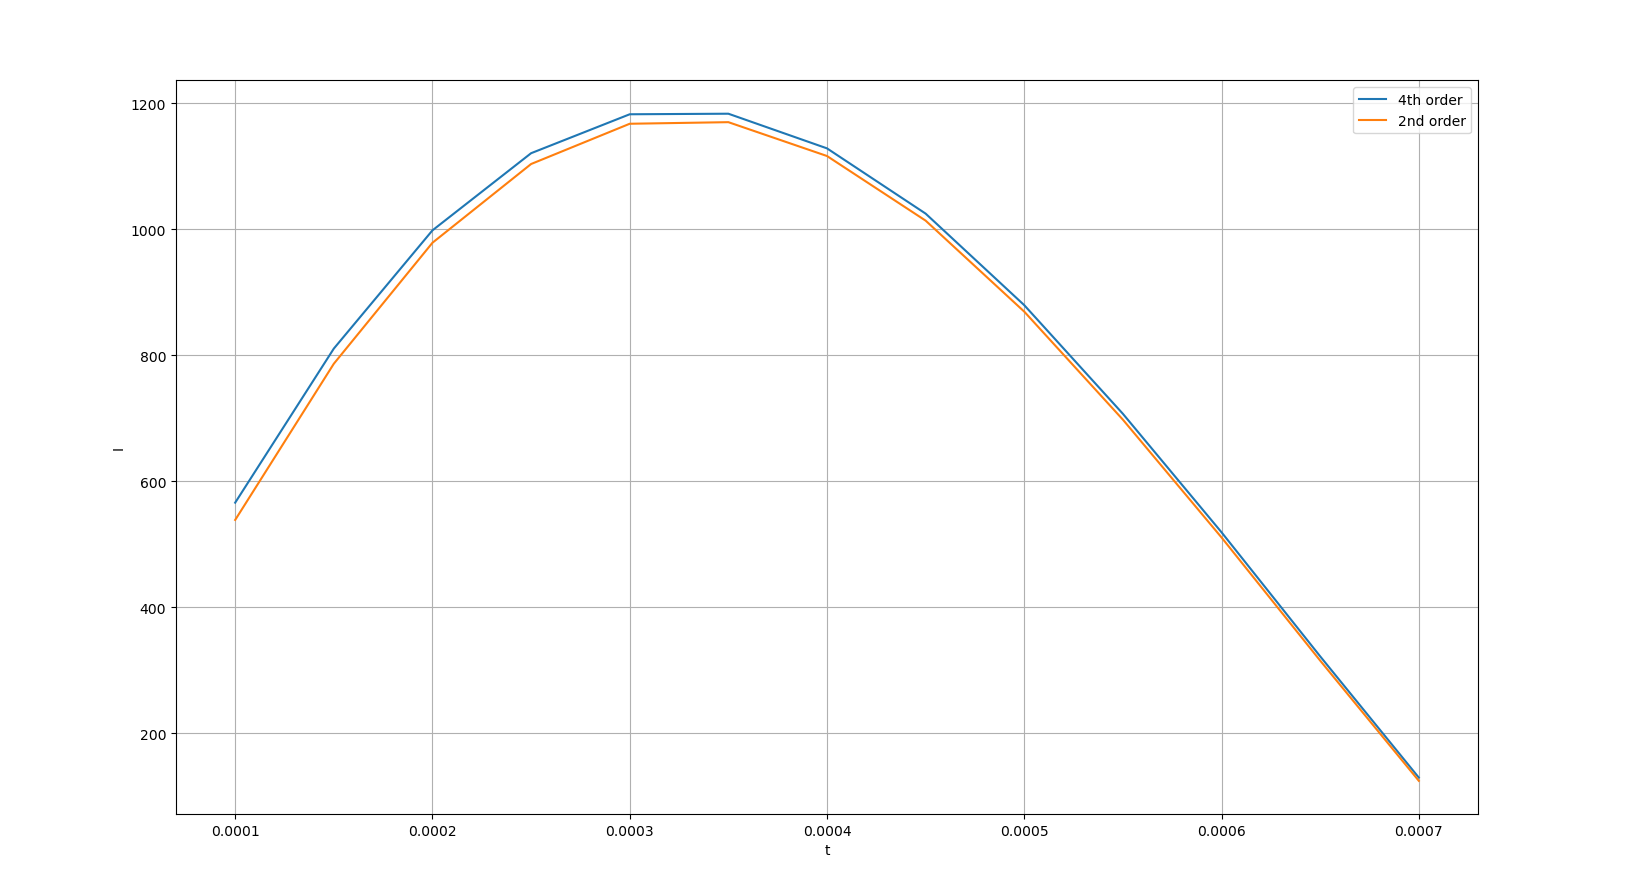
\includegraphics[width=\linewidth]{../1}
		\caption[I(t)]{I(t)}
		\label{fig:1}
	\end{figure}

	\begin{figure}[H]
		\centering
		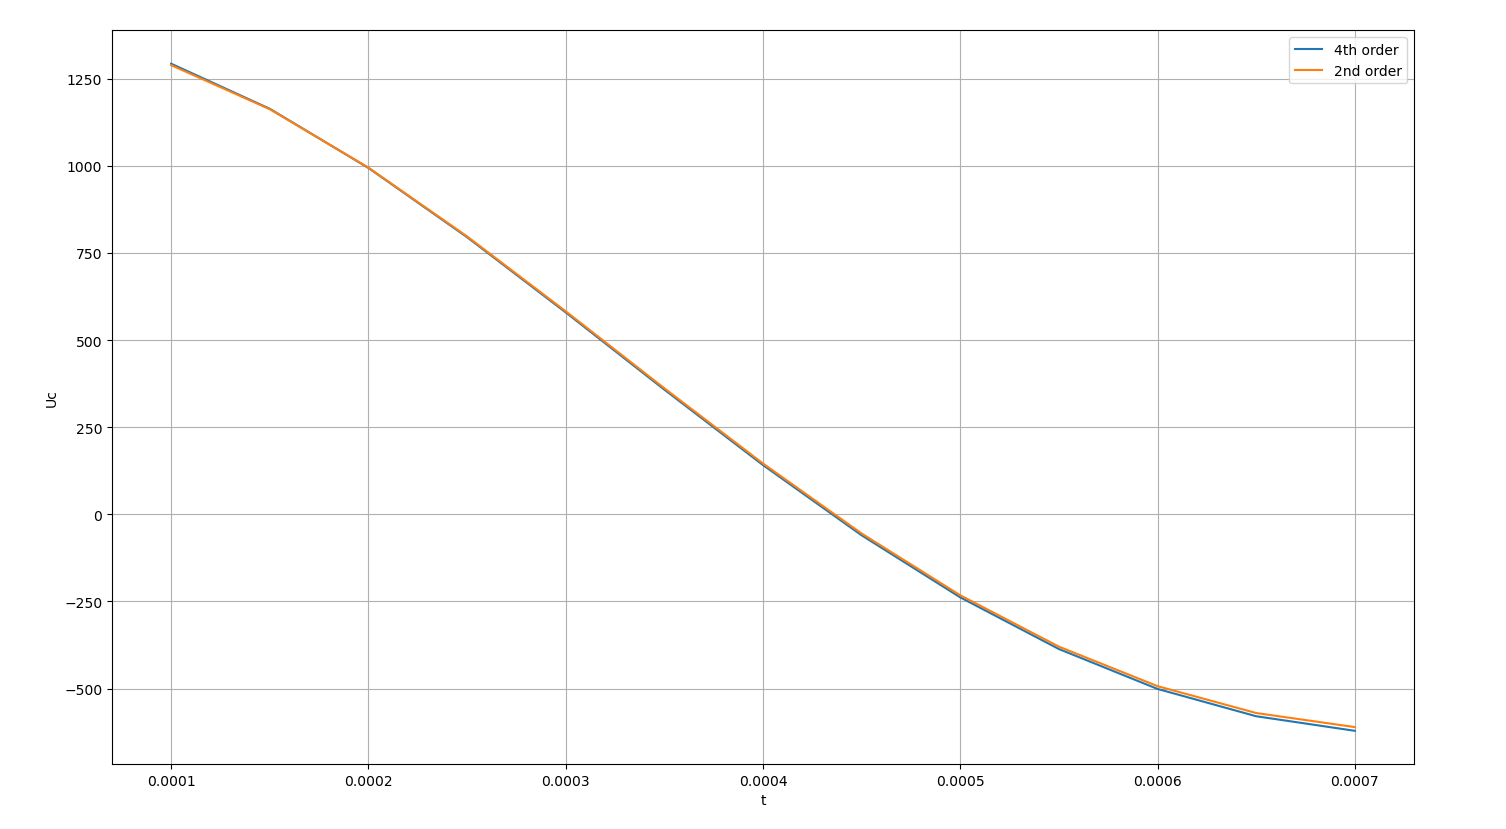
\includegraphics[width=\linewidth]{../2}
		\caption[U(t)]{U(t)}
		\label{fig:2}
	\end{figure}

	\begin{figure}[H]
		\centering
		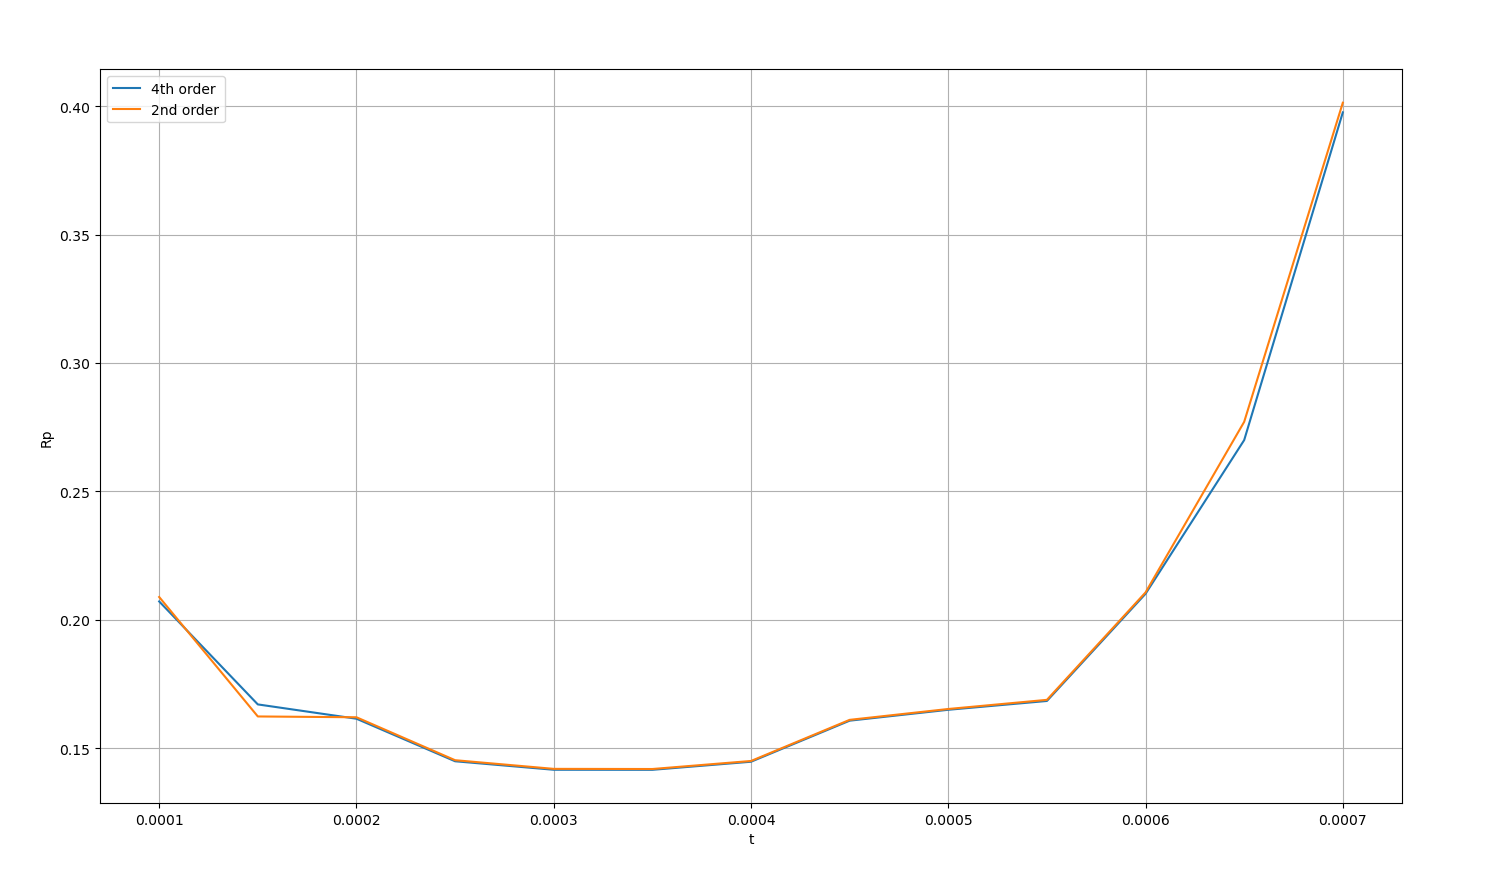
\includegraphics[width=\linewidth]{../3}
		\caption{Rp(t)}
		\label{fig:3}
	\end{figure}
	
	\begin{figure}[H]
		\centering
		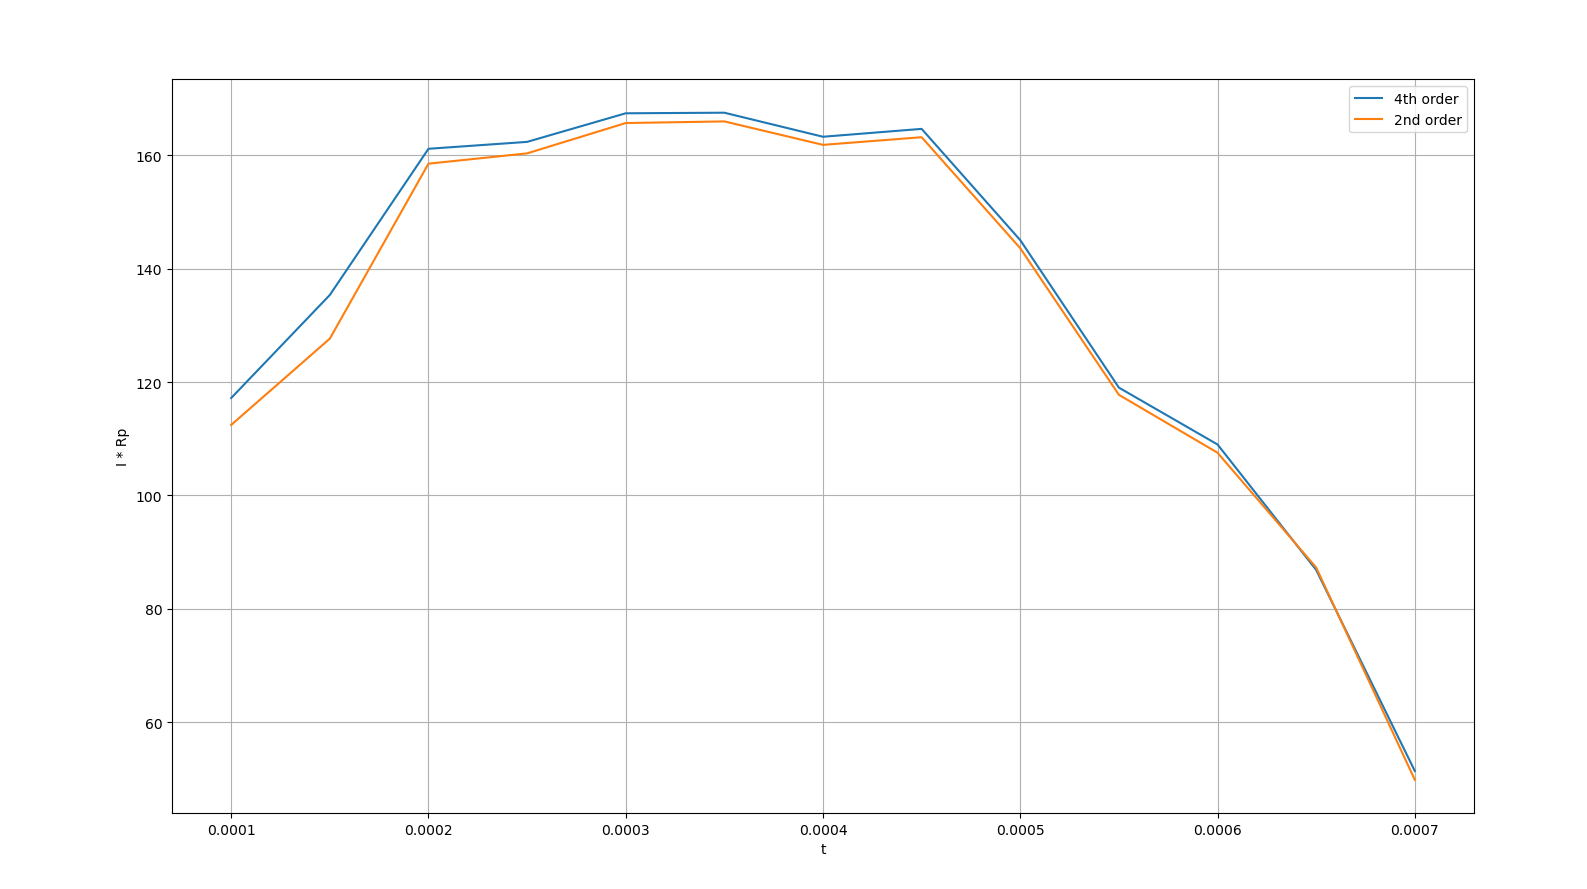
\includegraphics[width=\linewidth]{../4}
		\caption{I(t) * Rp(t)}
		\label{fig:4}
	\end{figure}

	 \begin{figure}[H]
	 	\centering
	 	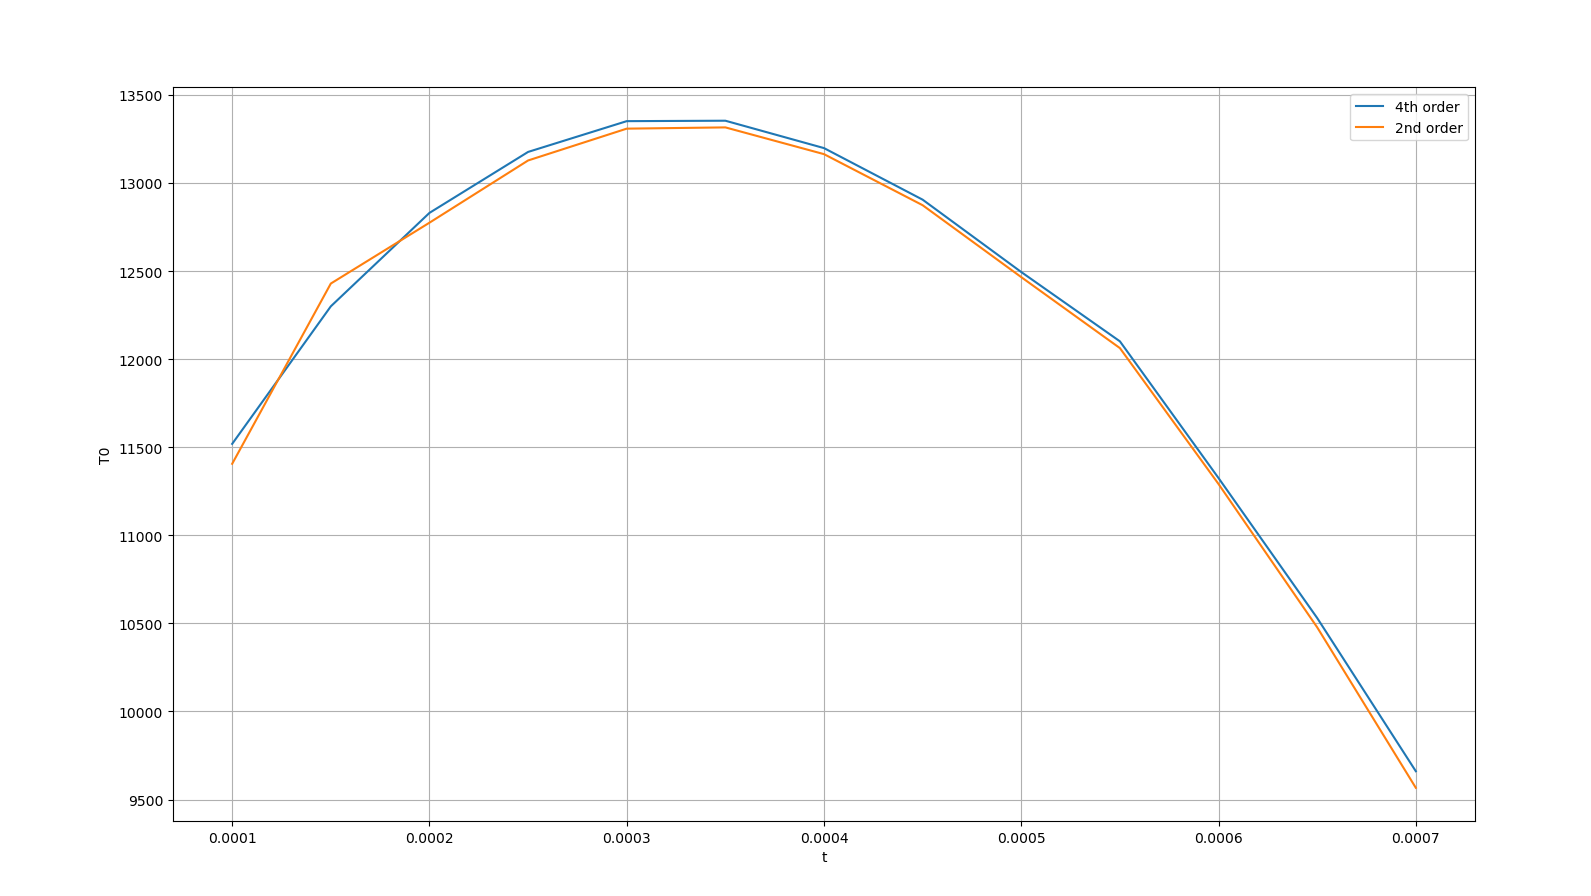
\includegraphics[width=\linewidth]{../6}
	 	\caption[T0(t)]{T0(t)}
	 	\label{fig:6}
	 \end{figure}
	 
\section{Вопросы и ответы}
	\begin{enumerate}
		\item \begin{enumerate}
			\item Вопрос: Какие способы тестирования программы можно предложить?
			\item Ответ: 1) Приравнять друг к другу знание Rk и Rp к 0. Потери в контуре будут отсутствовать. На графики будем видеть незатухающую синусоиду
			2) Сравнить результаты методов, с малым шагом
		\end{enumerate}
		\item \begin{enumerate}
			\item Вопрос: Получите систему разностных уравнений для решения
			сформулированной задачи неявным методом трапеций. Опишите
			алгоритм реализации полученных уравнений.
			\item Ответ:\begin{equation}
				\text{Возьмем систему:}
				\begin{cases}
					\frac{dl}{dt} & =\frac{U - (R_k + R_p(I))I}{L_k}\\
					\frac{dU}{dy} & =-\frac{I}{C_k}
				\end{cases}
				\text{Запишем выражение:}
			\end{equation}
			
			Запишем выражение:
			
			\begin{equation}
				I_{n+1} = I_n + \Delta t\frac{f(I_n, U_{n+1})}{2}
			\end{equation}
			\begin{equation}
				U_{n+1} = U_n + \Delta t\frac{g(l_n) + g(l_{n+1})}{2}
			\end{equation}
			
			Подставим выражение f и g:
			
			\begin{equation}
				l_{n + 1} = l_n + \Delta t\frac{U_n - (R_k + R_p(I_n))I_n + U_{n+1} - R_k + Rp(l_{n+1}))I_{n+1}}{2L_k}
			\end{equation}
			\begin{equation}
				U_{n+1} = U_n - \Delta\frac{l_n + l_{n+1}}{2C_k}
			\end{equation}
			
			Подставив $U_{n+1}$ из второго уравнения в первое, решим его относительно $l_{n+1}$
			
			\begin{equation}
				l_{n+1} = \frac{-2C_kR_p(I_n)I_n\Delta t + 4C_kI_kI_n - 2C_kI_nR_k\Delta t + 4C_kU_n\Delta t - I_n\Delta t^2}{den}
			\end{equation}
			
			Данное уравнение решается методом простых итераций $x^{(s)} = f(x^(s-1))$
			Получив $l_{n+1}$ подставим его значение в уравнение $U_{n+1} = U_n - \Delta t \frac{l_n + l_{n + 1}}{2C_k}$
			
		\end{enumerate}
		\item \begin{enumerate}
			\item Вопрос: Из каких соображений проводится выбор того или иного метода,
			учитывая, что чем выше порядок точности метода, тем он более сложен?

			\item Ответ: Все исходит из необходимых нам условий времени и точности вычисления результата.
			Точные методы требуют больше аппаратного времени на вычисление, в то время как их "коллеги" вычисляются быстрее, но с меньшей точностью.
			Нужно искать золотую середину.
			 
		\end{enumerate}
	\end{enumerate} 	
	
	
	
	
\end{document}
